\documentclass[a4paper,landscape,10pt]{article}
\usepackage[
  left=1.2cm,
  right=1.2cm,
  top=2.2cm,
  bottom=1.5cm,
  headheight=16pt,
  headsep=12pt
]{geometry}
\usepackage{longtable}
\usepackage{array}
\usepackage{amsmath}
\usepackage{ragged2e}
\usepackage{xcolor}
\usepackage{helvet}
\usepackage{colortbl}
\usepackage{fancyhdr}
\usepackage[hidelinks]{hyperref}
\usepackage{graphicx}

\renewcommand{\familydefault}{\sfdefault}
\pagestyle{fancy}
\fancyhf{}
\rhead{\footnotesize \textbf{GEMASTIK XIX 2026} -- Divisi Pengembangan Perangkat Lunak -- Tim Three Achilles (TRPL SV UGM)}
\lhead{\footnotesize \textbf{Storyboard Video Karya Akhir 100\% (Opsi Referensi Baru)}: Verifin}
\rfoot{\footnotesize Halaman \thepage}

\setlength{\parindent}{0pt}
\renewcommand{\arraystretch}{1.22}
\setlength{\tabcolsep}{3.5pt}

% Custom column types with clean wrapping and hyphenation
\newcolumntype{C}[1]{>{\Centering\arraybackslash}p{#1}}
\newcolumntype{L}[1]{>{\RaggedRight\arraybackslash}p{#1}}

\begin{document}

% Metadata Header
\noindent
\begin{minipage}[t]{0.68\textwidth}
{\large \textbf{GEMASTIK XIX 2026 -- Divisi Pengembangan Perangkat Lunak}} \\[0.15cm]
\small
\begin{tabular}{@{}lp{14.2cm}@{}}
\textbf{Pemeran (5)} & : 1. Rama (Alumni Muda), 2. Dr.Eng. Ir. Ganjar Alfian, S.T., M.Eng. (Dosen), 3. Matthew, 4. Hafidz, 5. Akmal (Three Achilles) \\
\textbf{Lokasi} & : \textbf{100\% Lingkungan Kampus} (Student Lounge, Selasar TILC, Ruang Dosen, \& Lab RPL TILC UGM) \\
\textbf{Properti} & : Smartphone (chat WA scam riil), Workstation Dual-Screen, Jas Almamater UGM \\
\textbf{Konsep} & : \textbf{Pragmatic-Cinematic \& Authentic Software Engineering} (Zero Heavy 3D Motion Graphics) \\
\end{tabular}
\end{minipage}
\hfill
\begin{minipage}[t]{0.30\textwidth}
\raggedleft
\small
\textbf{Target Durasi} : \textbf{08:50 (530 Detik)} (Batas Max: 10:00) \\
\textbf{Format Video} : MP4 1080p / 60fps \\
\textbf{Status Karya} : \textbf{\textcolor{green!50!black}{100\% Live Deployment}} \\
\textbf{Validasi} : \textbf{\textcolor{blue!70!black}{Kemitraan Resmi TRPL SV UGM}} \\
\end{minipage}

\vspace{0.25cm}
\begin{center}
{\Large \textbf{STORYBOARD PRODUKSI VIDEO KARYA AKHIR: ``VERIFIN'' (OPSI REFERENSI BARU)}} \\
\vspace{0.08cm}
{\small \textbf{Sistem Deteksi Lowongan Kerja Palsu Berbasis AI \& Multi-Source OSINT -- Alur Padat, Low-Motion, \& Naskah Tajam}}
\end{center}
\vspace{0.15cm}

\begin{longtable}{|C{1.3cm}|C{1.2cm}|L{1.8cm}|L{1.6cm}|L{1.9cm}|L{3.8cm}|L{8.8cm}|C{1.2cm}|L{3.2cm}|}
\hline
\rowcolor{gray!20}
\textbf{Scene} & \textbf{Int/Eks} & \textbf{Jenis Shoot} & \textbf{Camera Move} & \textbf{Audio} & \textbf{Visual} & \textbf{Deskripsi / Naskah} & \textbf{Durasi} & \textbf{Keterangan} \\
\hline
\endfirsthead

\hline
\rowcolor{gray!20}
\textbf{Scene} & \textbf{Int/Eks} & \textbf{Jenis Shoot} & \textbf{Camera Move} & \textbf{Audio} & \textbf{Visual} & \textbf{Deskripsi / Naskah} & \textbf{Durasi} & \textbf{Keterangan} \\
\hline
\endhead

\multicolumn{9}{|c|}{\cellcolor{gray!15}\textbf{BUMPER PEMBUKA}} \\
\hline
Bumper & - & Full Screen & Still & SFX Chime Logo & Logo Puspresnas, Kemendikbudristek, GEMASTIK XIX 2026, \& UGM & Tampilan pembuka resmi kompetisi GEMASTIK XIX 2026 dan Universitas Gadjah Mada dengan latar dark slate bersih. & 6 dtk & Clean fade in to scene 1 \\
\hline

\multicolumn{9}{|c|}{\cellcolor{gray!10}\textbf{BABAK I: THE REALITY, PSYCHOLOGICAL TRAP, \& THE DILEMMA (00:06 -- 01:45)}} \\
\hline
1 & Eks & Wide & Slow pan right & Ambience kampus & Fasad Gedung TILC SV UGM di waktu sore yang tenang & Suasana sore di kampus tempat mahasiswa dan alumni berkumpul. Membangun latar nyata lulusan baru. & 7 dtk & Establishing shot sinematik kampus UGM \\
\hline
2 & Int & Medium & Still & Ambience lounge & Meja Student Lounge TILC, laptop, Rama duduk melamun\par\vspace{3pt}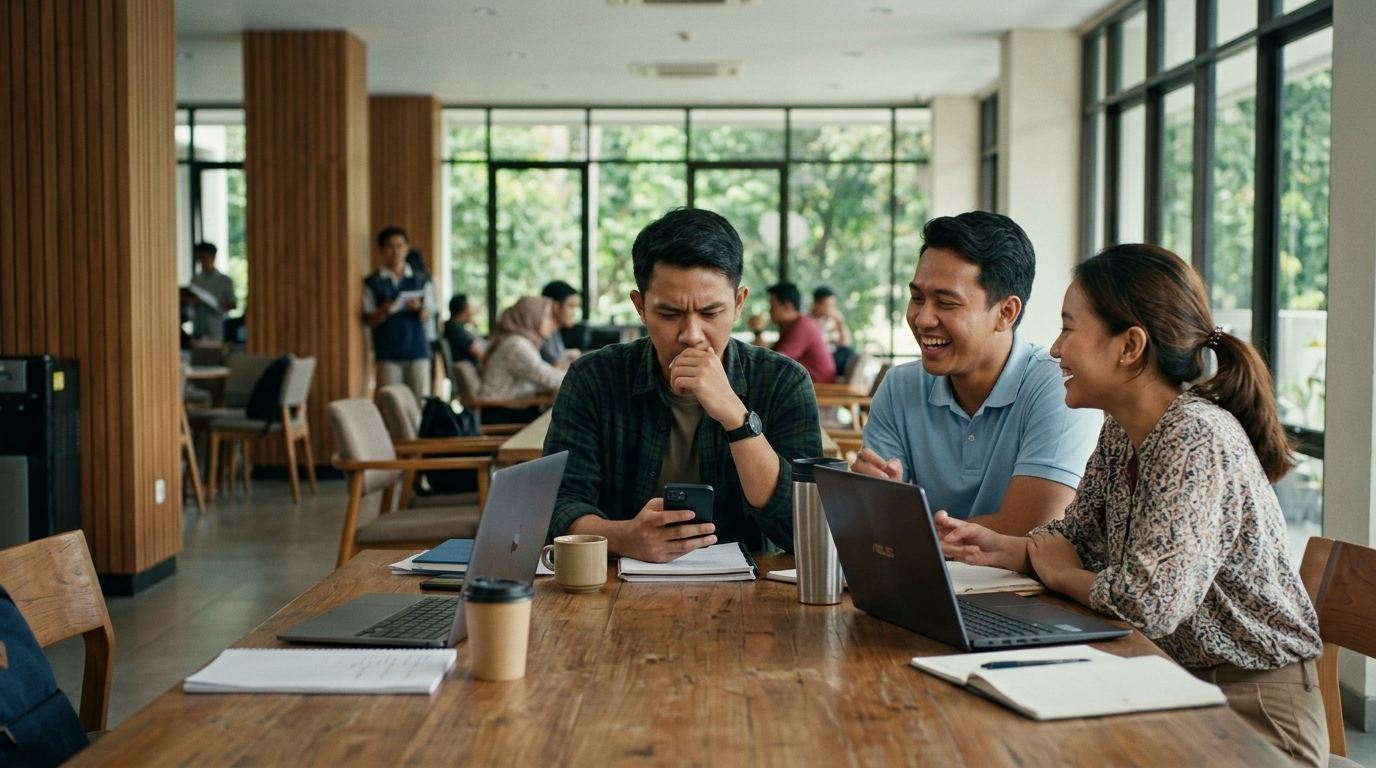
\includegraphics[width=\linewidth]{images/scene_2.jpg} & Rama duduk sendirian di sudut lounge, laptopnya terbuka menampilkan daftar lamaran kerja yang sepi respons. Rama menghela napas menatap layar HP-nya. & 9 dtk & Menyorot kesendirian dan beban pikiran lulusan baru \\
\hline
3 & Int & Over the Shoulder & Still & Ambience lounge & Layar smartphone Rama menampilkan chat WA mencurigakan & Kamera dari balik bahu menyorot pesan tawaran Admin WFH gaji 15 juta, namun wajib deposit seragam 500rb dan kirim selfie KTP. & 7 dtk & Focus pull dari bahu ke layar ponsel (crop jernih) \\
\hline
4 & Int & Close Up & Slow push-in & Monolog Rama & Wajah Rama membaca pesan dengan kening berkerut & \textbf{Rama (Monolog)}: ``Admin WFH gaji dua digit... Tapi kenapa baru tahap awal udah disuruh transfer lima ratus ribu buat uang seragam? Terus minta foto selfie KTP juga...'' & 12 dtk & Menyorot keraguan mendalam antara peluang dan kejanggalan \\
\hline
5 & Int & Medium Close Up & Still & Monolog Rama & Rama meletakkan HP di meja dan memegang keningnya & \textbf{Rama}: ``Aku udah empat bulan wisuda belum dapet kerja... Di satu sisi aku takut ini penipuan dan data KTP-ku disalahgunakan. Bukan cuma hilang lima ratus ribu, aku takut terseret sindikat kejahatan siber internasional. Tapi di sisi lain, aku takut nolak kalau ternyata ini beneran rezeki. Pas kondisi lagi terdesak begini, susah banget mikir jernih...'' & 14 dtk & Menyorot fenomena nyata \textit{Job-Seeker Desperation Bias} \\
\hline
6 & Int & Close Up to Med & Still & Monolog Rama & Rama mengambil HP dan berkasnya, beranjak berdiri & \textbf{Rama}: ``Nggak, aku nggak boleh gegabah ambil keputusan pas lagi panik. Mumpung lagi di kampus, lebih baik aku konsultasikan hal ini ke Pak Ganjar di ruang dosen.'' & 8 dtk & Sikap proaktif mencari verifikasi objektif ke dosen \\
\hline
7 & - & Split Screen & Still & Voiceover Hafidz & Layar kiri: B-roll Rama melangkah keluar lounge. Layar kanan: Kartu infografis data bersih & \textbf{Hafidz (VO)}: ``Data BPS mencatat lebih dari 7,2 juta pencari kerja di Indonesia. Riset GASA membuktikan 49\% korban penipuan digital berawal dari modus loker fiktif dengan kerugian Rp49 triliun. Bukan sekadar kerugian uang lima ratus ribu, modus loker fiktif kini menjadi pintu gerbang utama Tindak Pidana Perdagangan Orang (TPPO) ke sindikat kejahatan siber regional yang telah menjerat lebih dari 3.300 WNI. Dalam tekanan ekonomi, bias keputusasaan melumpuhkan logika kritis para korban.'' & 20 dtk & Infografis 2D minimalis elegan (tanpa 3D orbit) \\
\hline
8 & - & Full Screen & Fade in & SFX Sub-bass whoosh & Title card elegan: VERIFIN: Garda Talenta Digital & Teks bersih pada dark navy: \par\vspace{2pt} \textbf{VERIFIN: GARDA TALENTA DIGITAL} \par\vspace{1pt} \textit{Sistem Deteksi Loker Palsu Berbasis AI \& Multi-Source OSINT} \par\vspace{1pt} Three Achilles -- TRPL SV UGM & 9 dtk & Title reveal profesional dan berwibawa \\
\hline

\multicolumn{9}{|c|}{\cellcolor{gray!10}\textbf{BABAK II: THE BRIDGE \& COGNITIVE INTERVENTION (01:45 -- 02:45)}} \\
\hline
9 & Int & Medium & Track in & Ambience tenang & Rama mengetuk dan memasuki ruang dosen TILC & \textbf{Rama}: ``Permisi, Pak Ganjar... Maaf mengganggu waktunya, Pak. Saya ingin berkonsultasi sebentar soal tawaran kerja yang baru saja saya terima.'' \par\vspace{2pt} \textbf{Pak Ganjar}: ``Silakan masuk, Rama. Duduk dulu, ada apa?'' & 9 dtk & Framing rapi di ruang kerja dosen \\
\hline
10 & Int & Two Shot & Still & Dialog Rama \& Pak Ganjar & Pak Ganjar dan Rama duduk berhadapan & \textbf{Rama}: ``Saya bimbang banget, Pak Ganjar. Format pesannya rapi mencatut nama perusahaan besar, tapi mereka mewajibkan transfer uang registrasi. Saya takut salah ambil keputusan karena panik butuh kerja.'' & 10 dtk & Dialog konsultasi hangat dosen-mahasiswa \\
\hline
11 & Int & Medium Close Up & Still & Dialog Pak Ganjar & Pak Ganjar tersenyum menenangkan dan memberi arahan solusi\par\vspace{3pt}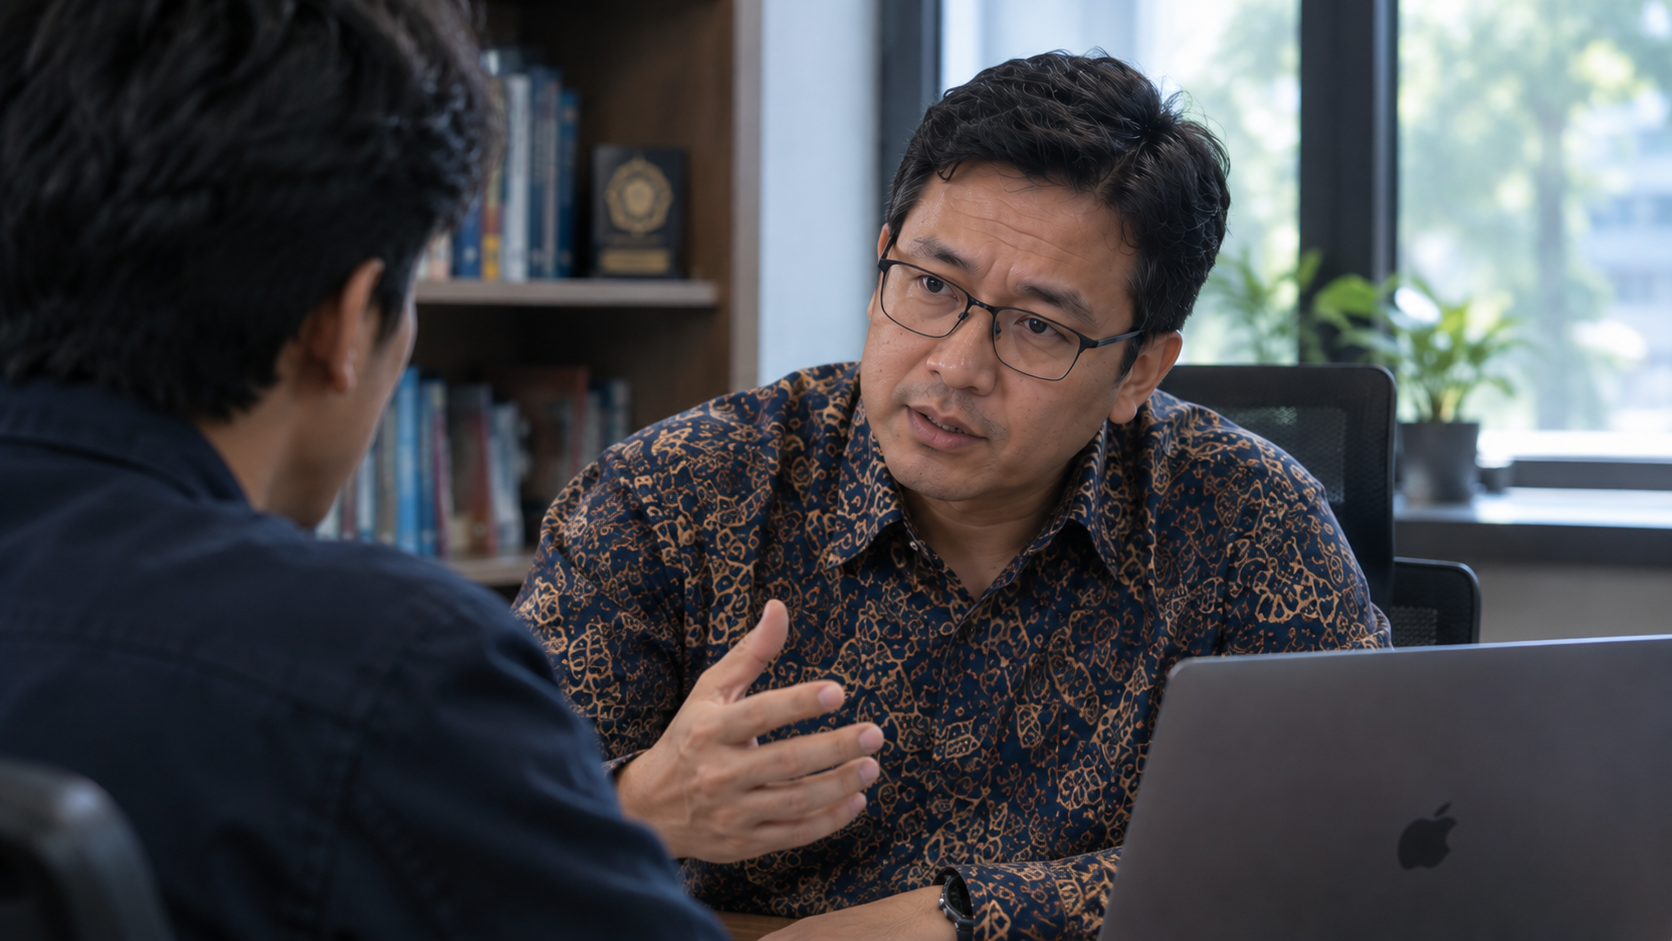
\includegraphics[width=\linewidth]{images/scene_12.png} & \textbf{Pak Ganjar}: ``Keputusan kamu tepat untuk berhenti sejenak dan tidak langsung transfer, Rama. Sesuai \textbf{Pasal 38 Permenaker Nomor 39 Tahun 2016}, pemberi kerja dilarang keras memungut biaya penempatan dalam bentuk apa pun kepada pencari kerja. Sindikat memang sengaja mengeksploitasi kepanikan pelamar. Kamu butuh bukti forensik digital yang objektif. Kebetulan sekali, rekan-rekanmu di TRPL SV UGM sudah meluncurkan \textbf{Verifin} sebagai jeda kognitif berbasis AI dan OSINT. Sistemnya sudah live 100\%, ayo kita buktikan langsung di lab.'' & 25 dtk & Menghubungkan dasar hukum Permenaker ke solusi teknologi \\
\hline
12 & Eks & Medium & Tracking walk & Ambience selasar & Pak Ganjar dan Rama berjalan di selasar lantai 2 TILC & Pak Ganjar dan Rama berjalan melintasi selasar modern kampus TILC menuju Lab Rekayasa Perangkat Lunak. & 8 dtk & Transisi dinamis menghubungkan dua lokasi \\
\hline
13 & Int & Wide & Pan left & Ambience lab & Lab Software Engineering TRPL SV UGM & \textbf{Pak Ganjar}: ``Halo rekan-rekan Three Achilles. Ini Rama ingin memverifikasi tawaran loker yang mencurigakan.'' \par\vspace{2pt} \textbf{Matthew}: ``Halo Mas Rama, selamat siang Pak Ganjar! Pas banget, Verifin saat ini sudah live dan siap kita uji langsung secara real-time. Yuk langsung kita bedah!'' & 14 dtk & Menampilkan ruang lab riil dan kesiapan tim \\
\hline

\multicolumn{9}{|c|}{\cellcolor{gray!10}\textbf{BABAK III: THE BATTLE OF EDGE CASES -- LIVE DEMO 100\% (3 KANAL INPUT) (02:45 -- 06:15)}} \\
\hline
14 & Int & Over the Shoulder & Still & Dialog Tim \& Rama & Rama duduk di depan workstation, Matthew mendampingi & \textbf{Matthew}: ``Platform kami menyediakan \textbf{3 Kanal Input Utama}: Input Tautan (URL), Input Teks pesan, dan Input Gambar atau Poster via OCR. Mas Rama dapat tawaran lokernya lewat apa saja? Kita uji satu per satu!'' \par\vspace{2pt} \textbf{Rama}: ``Ini Mas, di ponselku ada tautan situs rekrutmen BUMN, pesan forward chat teks toko motor, sama tangkapan layar brosur kerja.'' & 14 dtk & Menegaskan ketersediaan 3 kanal input resmi \\
\hline
15 & Int & Screen Capture & Still & SFX Typing \& Klik & Layar browser live verifin.app (Kanal 1: Input Tautan) & Tab \textbf{Kanal 1: Input Tautan (URL)} dipilih. Rama menempelkan tautan \texttt{https://recruitment-semenindonesia.xyz} (mencatut BUMN Semen Indonesia) dan menekan tombol ``Analisis Lowongan''. \par\vspace{2pt} \textbf{VO (Matthew)}: ``Pada kanal pertama, pengguna dapat memverifikasi tautan web rekrutmen atau formulir online yang mencurigakan secara instan.'' & 11 dtk & Screen recording 1080p jernih, responsif tanpa lag \\
\hline
16 & - & Screen Capture & Still & SFX Alert Ping & Dashboard Hasil: Trust Score Gauge berputar ke 94/100 (Badge Merah)\par\vspace{3pt}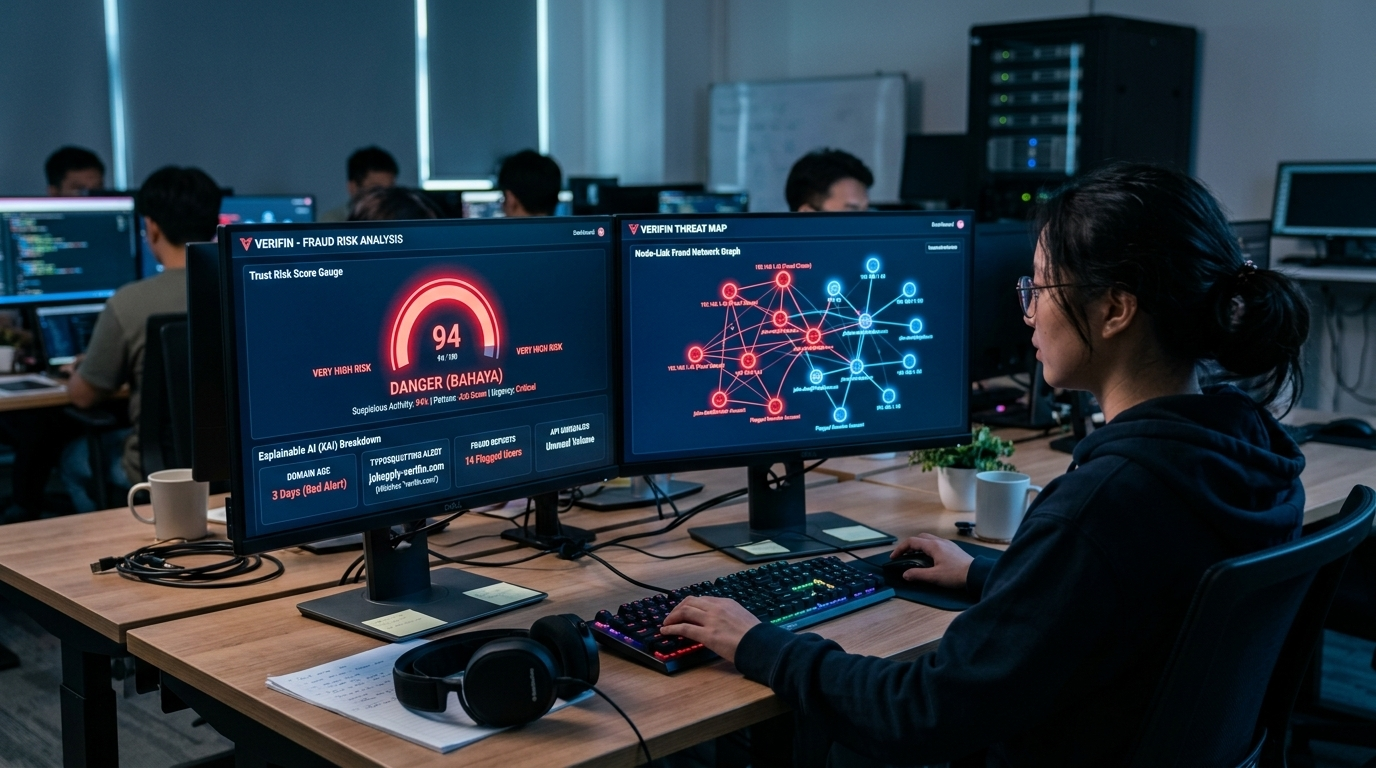
\includegraphics[width=\linewidth]{images/scene_20.jpg} & \textbf{Akmal}: ``Hasil analisis keluar dalam 1,8 detik. Sistem menetapkan skor risiko 94 dari 100 dengan vonis BAHAYA TINGGI!'' \par\vspace{2pt} Dashboard Hasil Instan: Skor Risiko 94/100 (WASPADA PENIPUAN). \newline Kartu Bukti XAI Merah: \newline $\bullet$ Domain Age: 5 Hari (Penalti +30) \newline $\bullet$ Typosquatting .xyz vs Resmi .co.id \newline $\bullet$ Pelanggaran Hukum: Pasal 38 Permenaker No. 39/2016 \newline $\bullet$ Biro Travel: 14 Laporan Fraud di Kredibel.id & 15 dtk & Worst-Case FAKE terbongkar tuntas secara ilmiah \\
\hline
17 & Int & Medium & Still & Dialog Matthew \& Rama & Matthew menunjuk rincian bukti forensik digital pada monitor\par\vspace{3pt}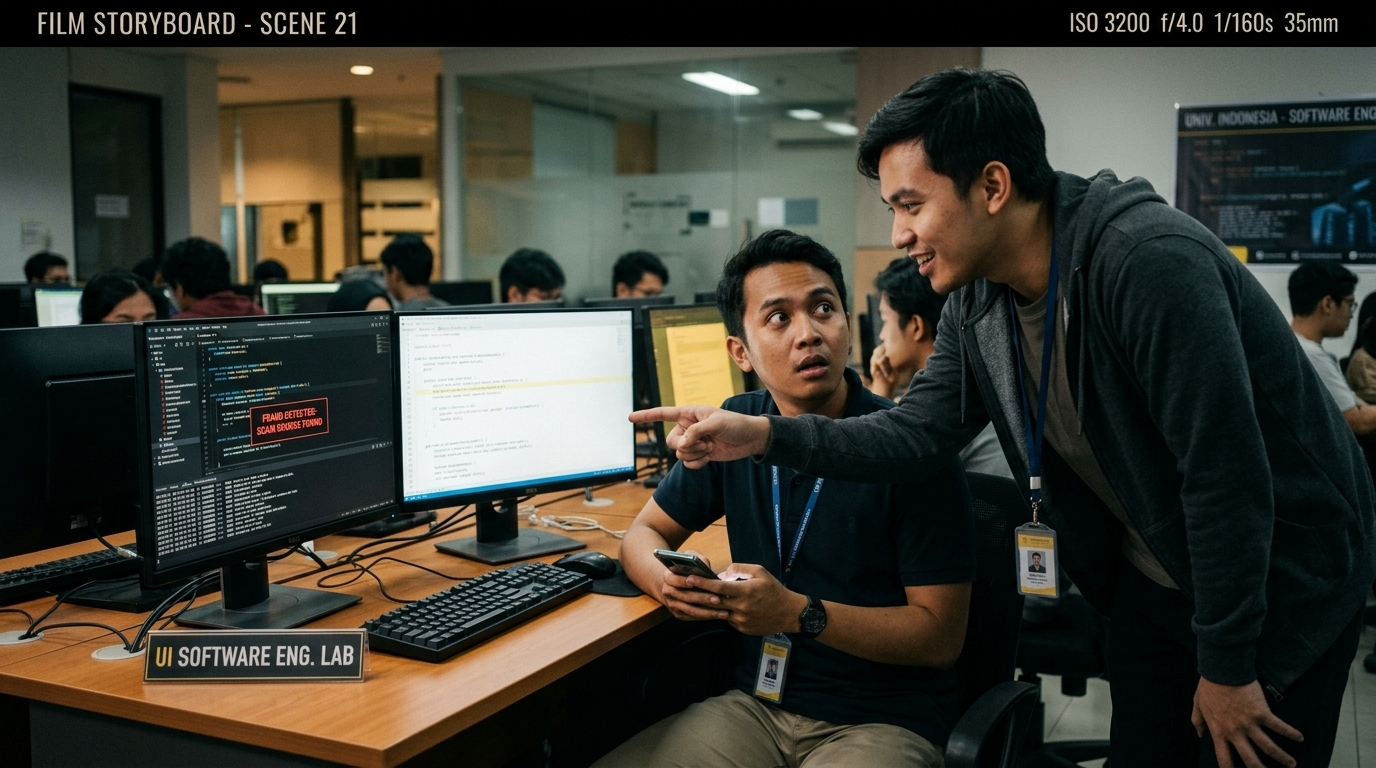
\includegraphics[width=\linewidth]{images/scene_21.jpg} & \textbf{Matthew}: ``Inilah keunggulan sistem kami yang \textbf{non-blackbox}, Mas Rama. Kami tidak sekadar memberikan vonis tanpa alasan seperti chatbot biasa, melainkan menyajikan rincian kartu bukti yang transparan: Pertama, domain ini baru dibuat 5 hari lalu. Kedua, terjadi typosquatting domain palsu .xyz. Dan ketiga, kewajiban transfer tiket biro travel melanggar mutlak \textbf{Pasal 38 Permenaker No. 39 Tahun 2016}, ditambah kontaknya memiliki 14 laporan penipuan di Kredibel!'' \par\vspace{2pt} \textbf{Rama}: ``Ya ampun... Kalau tadi aku cuma percaya tampilan web yang rapi doang, uang lima ratus ribu punyaku pasti langsung melayang!'' & 25 dtk & Penjelasan transparansi non-blackbox XAI \& rujukan hukum \\
\hline
18 & Int & Screen Capture & Pan / Click & SFX Click Tab & Tab Fraud Network Graph dibuka & Kursor mengklik tab Fraud Network Graph. Graf interaktif (React Flow + D3.js) menampilkan node nomor telepon penipu menyala merah dan terhubung ke 3 sindikat PT fiktif lainnya di database. & 18 dtk & Bukti intelijen data grafis sindikat riil \\
\hline
19 & Int & Medium & Still & Dialog Hafidz & Hafidz menjelaskan kecerdasan graf sindikat & \textbf{Hafidz}: ``Verifin tidak bekerja terisolasi. Melalui Fraud Network Graph, sistem memetakan korelasi entitas. Nomor ini terbukti terkoneksi ke sindikat penipuan yang sama di beberapa kota dengan modus tiket serupa.'' & 16 dtk & Penjelasan kecerdasan graf lintas platform \\
\hline
20 & Int & Close Up & Still & Dialog Rama & Rama menunjukkan chat kedua di ponselnya & \textbf{Rama}: ``Bener-bener membuka mata aku... Tapi gimana dengan kasus kedua ini Mas? Ada broadcast loker toko variasi motor lokal di Jogja (The Biker Shop), tapi daftarnya disuruh isi Google Form dan kontaknya cuma pakai email Gmail gratisan (hrdthebikershop@gmail.com). Ini jangan-jangan penipuan juga?'' & 16 dtk & Transisi ke Kanal 2: Anti-False Positive pesan teks \\
\hline
21 & Int & Screen Capture & Still & SFX Processing & Kanal 2: Input Teks Verifin diuji & Rama beralih ke tab \textbf{Kanal 2: Input Teks}. Teks broadcast loker The Biker Shop disalin dari HP dan diinput ke kolom teks Verifin. Tombol analisis diklik. & 6 dtk & Demo pemrosesan kanal input teks secara real-time \\
\hline
22 & - & Screen Capture & Still & SFX Success Ping & Dashboard Hasil: Skor Risiko 12/100, Badge Hijau (AMAN \& TERVALIDASI) & \textbf{Akmal}: ``Lihat perbedaannya, Mas Rama. Sistem Verifin tidak serta-merta memvonis merah hanya karena loker menggunakan email Gmail gratisan.'' \par\vspace{2pt} Dashboard Hasil (Skor Risiko: 12/100, AMAN \& TERVALIDASI): \newline $\bullet$ Alamat Fisik Valid: Jl. Parangtritis No. 38 (OpenStreetMap) \newline $\bullet$ Medsos Aktif: IG @thebikershop.jogja (1.6K Followers) \newline $\bullet$ Klausul Finansial: Bebas Biaya (Patuh Permenaker No. 39/2016, Penalti 0) & 16 dtk & Visualisasi kontras melegakan: Merah ke Hijau \\
\hline
23 & Int & Medium & Still & Dialog Akmal \& Hafidz & Akmal dan Hafidz menjelaskan di depan monitor & \textbf{Akmal}: ``Inilah inovasi Anti-False Positive Verifin. Sistem kami tidak sembarangan memvonis merah hanya karena email Gmail. Mesin OSINT mengecek keberadaan fisik toko melalui OpenStreetMap, mengonfirmasi aktivitas media sosial usahanya, dan memastikan kepatuhan penuh terhadap Permenaker tanpa pungutan biaya liar.'' \par\vspace{2pt} \textbf{Hafidz}: ``Dengan begitu, reputasi bisnis UMKM lokal tetap terjaga dan pencari kerja tidak kehilangan kesempatan kerja yang sah.'' \par\vspace{2pt} \textbf{Rama}: ``Wah, adil banget! Jadi aku nggak perlu cemas atau ragu lagi buat melamar ke toko ini.'' & 25 dtk & Membuktikan keadilan sistem (Fairness \& Reliability) \\
\hline
24 & Int & Screen Capture & Still & SFX Shutter & Kanal 3: Input Gambar / Poster (OCR) & Tab \textbf{Kanal 3: Input Gambar / Poster} dipilih. Tangkapan layar poster loker diunggah. Engine PaddleOCR 2.8 mengekstrak teks otomatis dan menganalisis risiko dalam hitungan detik. \par\vspace{2pt} \textbf{Matthew}: ``Kanal ketiga kami dirancang khusus untuk gambar poster loker. Dengan PaddleOCR 2.8, sistem mengekstrak teks otomatis dari tangkapan layar ponsel bahkan dari gambar buram sekalipun.'' & 18 dtk & Memperlihatkan kelengkapan 3 kanal input (URL, Teks, OCR) \\
\hline
25 & Int & Screen Capture & Still & SFX Click FAB & Tombol Floating Action Button ``[!] Laporkan Loker'' diklik & Kursor mengklik FAB oranye kontras di pojok kanan bawah. Form pelaporan terisi otomatis dan tersinkronisasi ke Community Feed Real-Time untuk melindungi sesama pelamar. \par\vspace{2pt} \textbf{VO (Matthew)}: ``Ketika pengguna menemukan pola penipuan baru, satu klik pada tombol Lapor Komunitas langsung menyinkronkan bukti ke basis data kolektif real-time.'' & 17 dtk & Demo pertahanan komunitas hasil evaluasi testing \\
\hline

\multicolumn{9}{|c|}{\cellcolor{gray!10}\textbf{BABAK IV: SOFTWARE ENGINEERING EXCELLENCE \& VALIDASI (06:15 -- 07:55)}} \\
\hline
26 & Int & Medium Two Shot & Still & Dialog Hafidz \& Matthew & Hafidz dan Matthew memaparkan arsitektur di depan monitor lab & \textbf{Hafidz}: ``Verifin dikembangkan menggunakan metodologi Agile Scrum dalam 4 Sprint terukur, didukung alur kerja CI/CD otomatis. Di balik antarmuka yang sederhana, Verifin dibangun di atas pipeline rekayasa multi-layer yang kokoh: Layer 1 Hybrid NER, Layer 2 Fast NLP Classifier, Layer 3 Parallel Async OSINT, Layer 4 Graph Reasoning, hingga Layer 5 Additive Explainable AI. Verifin secara tegas menolak model AI kotak hitam (\textit{blackbox}). Kami menggunakan formulasi matematis terkalibrasi $S_{\text{risiko}} = S_{\text{dasar}} + \sum \phi_i$, di mana setiap bobot $\phi_i$ diturunkan dari bukti objektif dan hukum ketenagakerjaan, bukan sekadar halusinasi probabilitas teks.'' & 28 dtk & Penjelasan Agile Scrum \& non-blackbox XAI \\
\hline
27 & - & Screen Capture & Still & SFX Typing Terminal & Rekaman layar eksekusi automated test \& metrik rekayasa & \textbf{Matthew (VO)}: ``Kualitas perangkat lunak dijamin melalui pengujian otomatis dengan code coverage mencapai 91\% dan skor ROC-AUC 0,996 pada dataset EMSCAD. Seluruh layanan di-containerize dengan arsitektur mikro terisolasi menggunakan Next.js 16 dan FastAPI yang beroperasi stabil dengan latensi rata-rata di bawah dua detik.'' \par\vspace{2pt} Rekaman Layar Eksekusi Terminal \& Metrik: \newline $\bullet$ Automated test: pytest tests/ -v $\rightarrow$ \textbf{100\% PASSED} (Coverage 91\%) \newline $\bullet$ Model ML: ROC-AUC mencapai \textbf{0,996} pada dataset EMSCAD \newline $\bullet$ Latensi respons FastAPI di bawah 2 detik \newline $\bullet$ Live deployment terisolasi di Dokploy \& Cloudflare Tunnel & 22 dtk & Pembuktian software engineering tangguh \& riil \\
\hline
28 & Int & Medium & Still & Dialog Akmal \& Matthew & Akmal dan Matthew memegang dokumen pengujian \& kemitraan prodi & \textbf{Akmal}: ``Verifin telah diuji melalui controlled pilot study pada pencari kerja riil. Hasilnya luar biasa: efisiensi waktu investigasi mencapai 93,5\%---dari rata-rata 18,4 menit terpangkas menjadi hanya 1,2 menit! Akurasi deteksi bahaya melonjak dari 45\% menjadi 95\%, dengan skor System Usability Scale (SUS) 83,5 berkategori Excellent Grade A!'' \par\vspace{2pt} \textbf{Matthew}: ``Lebih dari itu, sistem ini telah mendapatkan validasi institusional melalui kemitraan resmi dengan Program Studi TRPL Sekolah Vokasi UGM. Ke depan, Verifin dirancang beroperasi berkelanjutan mendukung SDGs Poin 8: Pekerjaan Layak dan Pertumbuhan Ekonomi, memperluas integrasi API publik bagi pusat karir universitas dan Disnakertrans secara nasional.'' & 22 dtk & Validasi empiris (SUS 83,5) \& SDGs Poin 8 \\
\hline

\multicolumn{9}{|c|}{\cellcolor{gray!10}\textbf{BABAK V: RESOLUTION, EMPOWERMENT, \& CLOSING CALL (07:55 -- 08:50)}} \\
\hline
29 & Int & Two Shot & Still & Dialog Pak Ganjar & Pak Ganjar menepuk bahu Rama di Lab RPL dan tersenyum bangga\par\vspace{3pt}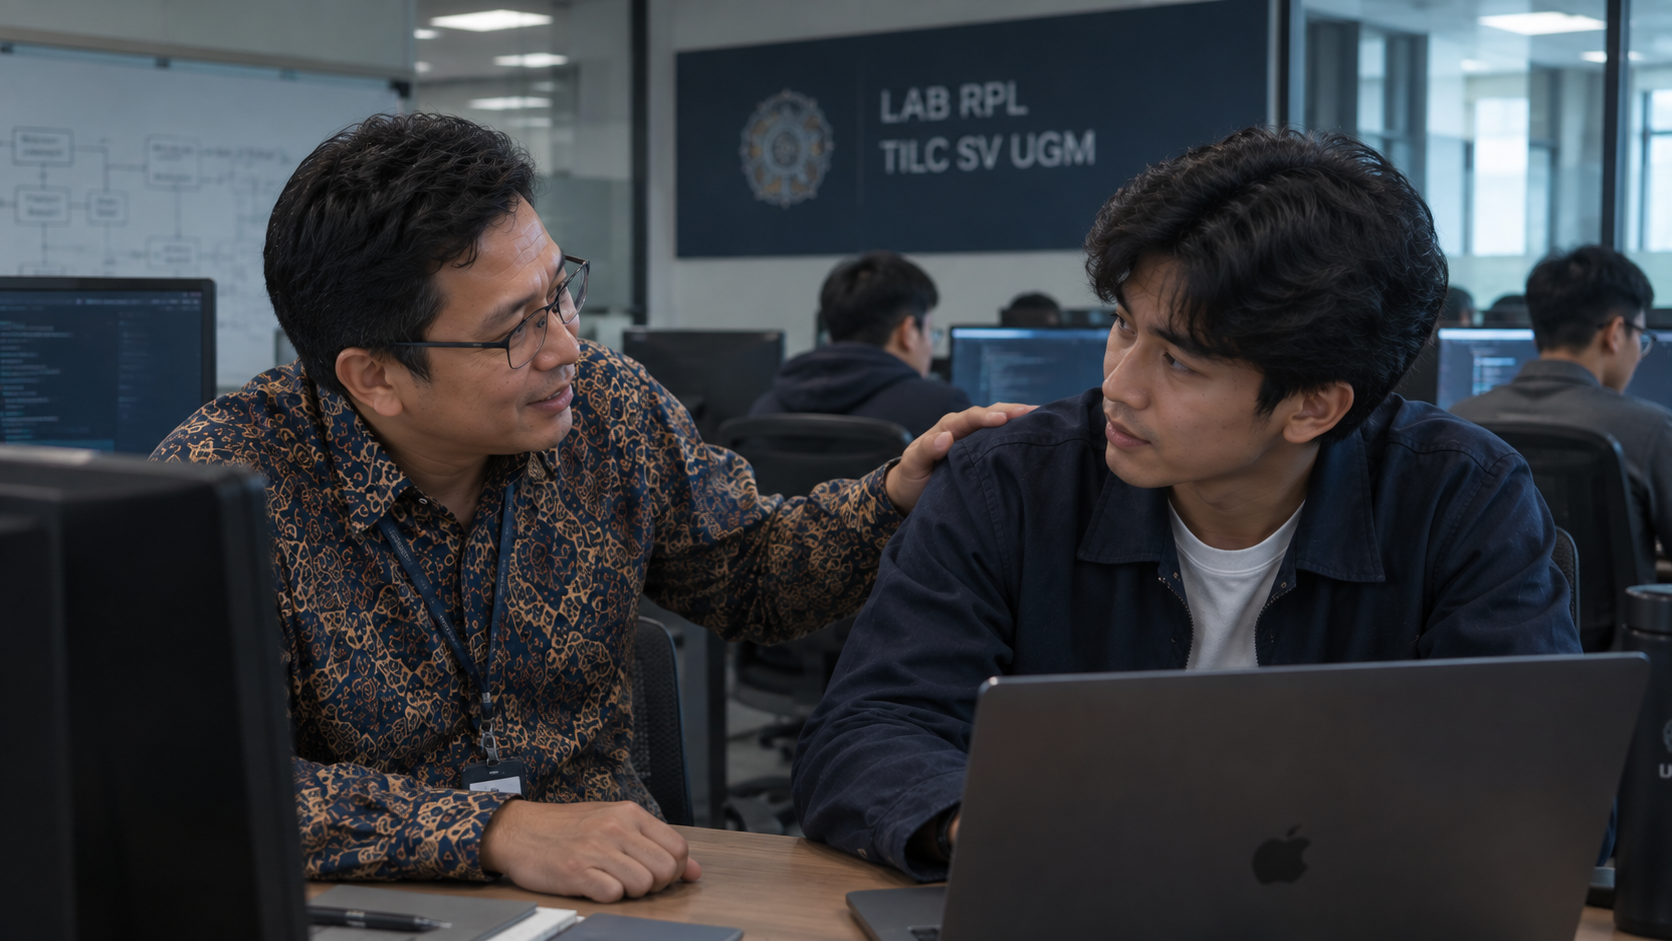
\includegraphics[width=\linewidth]{images/scene_35.png} & \textbf{Pak Ganjar}: ``Inilah esensi sejati dari rekayasa perangkat lunak. Bukan sekadar merangkai baris kode, tetapi menghadirkan solusi teknologi yang melindungi harkat dan masa depan generasi muda Indonesia dari jeratan kejahatan siber.'' & 15 dtk & Apresiasi akademis \& etika profesi rekayasa \\
\hline
30 & Int & Close Up & Still & Dialog Rama & Rama membuka web Verifin di browser smartphone-nya & \textbf{Rama}: ``Terima kasih banyak Pak Ganjar dan tim Verifin! Sekarang rasanya bener-bener plong dan aman. Cukup sekali cek di Verifin, aku bisa melamar kerja dengan tenang tanpa takut terjebak penipuan.'' & 13 dtk & Resolusi kepraktisan mobile web \& ketenangan batin \\
\hline
31 & Eks & Medium Tracking & Slow dolly back & Music Up (Heroic) & Kelima pemeran melangkah di selasar megah TILC SV UGM\par\vspace{3pt}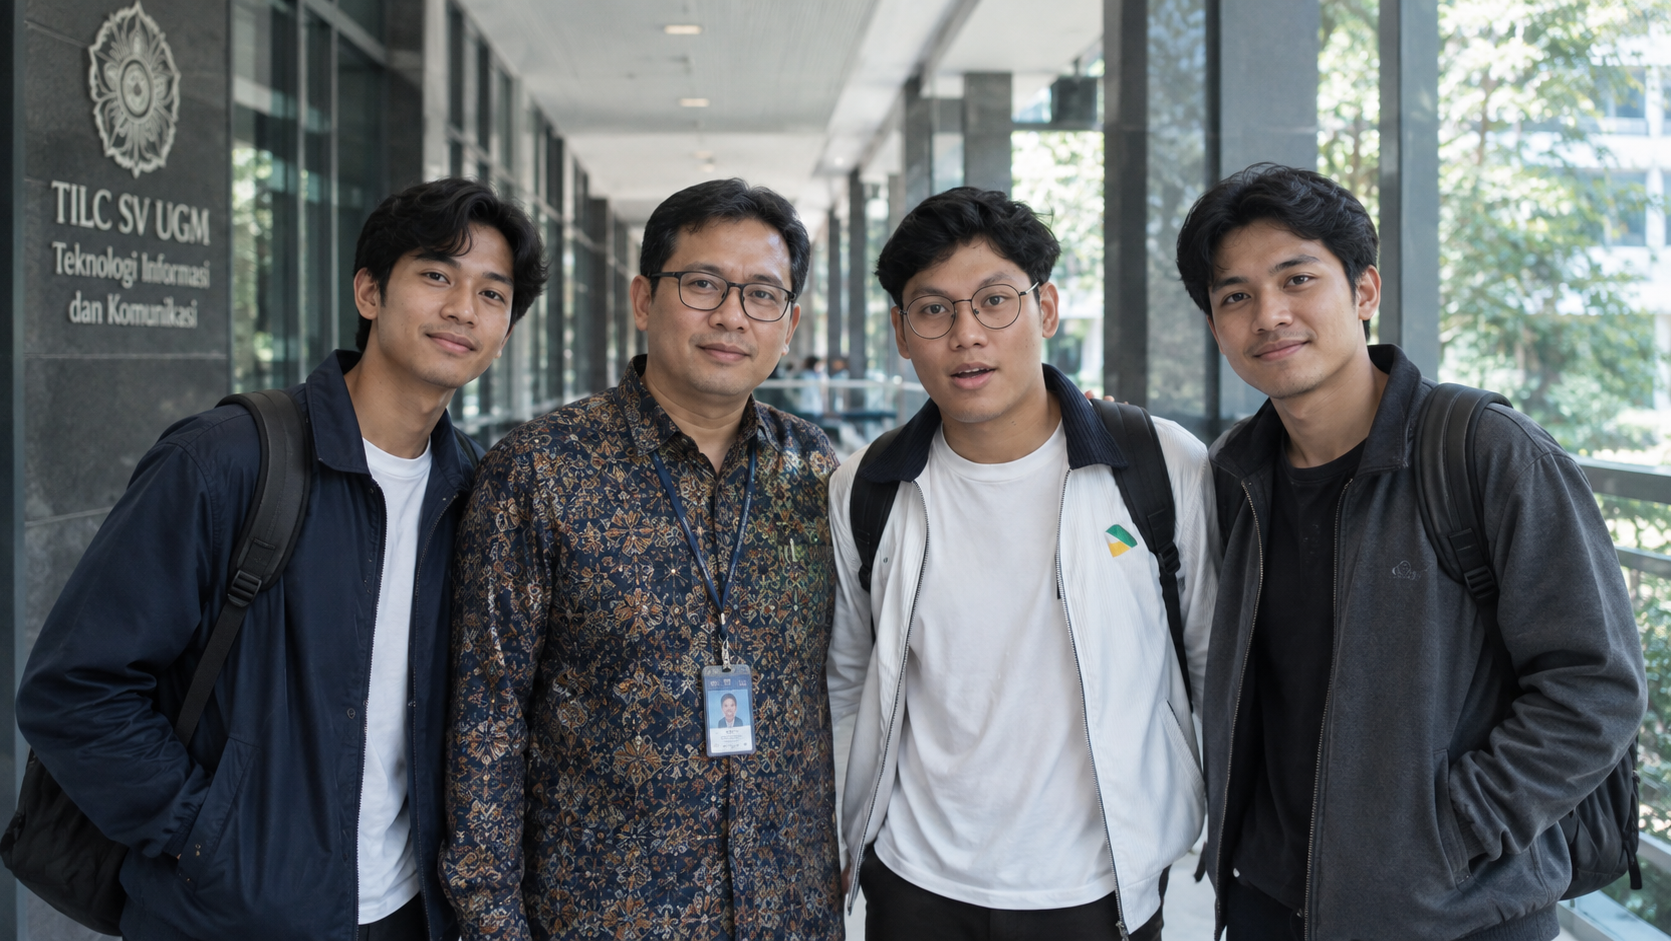
\includegraphics[width=\linewidth]{images/scene_37.png} & Kelima pemeran (Rama, Pak Ganjar, Hafidz, Matthew, Akmal) mengenakan jas almamater UGM melangkah mantap di selasar kampus megah di bawah sinar matahari hangat. & 10 dtk & Visual sinematik klimaks kampus \\
\hline
32 & Eks & Medium & Still & Orasi Penutup Tim & Kamera menyorot kelima pemeran & \textbf{Hafidz}: ``Bagi jutaan pemuda Indonesia, lowongan kerja adalah gerbang masa depan, bukan perangkap keputusasaan.'' \newline \textbf{Matthew}: ``Verifin hadir sebagai garda terdepan, membentengi talenta bangsa dengan kecerdasan data dan transparansi.'' \newline \textbf{Akmal}: ``Sebuah karya rekayasa perangkat lunak dari Sekolah Vokasi UGM untuk Indonesia yang aman dan berdaya.'' \newline \textbf{Semua Bersama}: ``Kami Tim Three Achilles, siap mengawal talenta bangsa di GEMASTIK XIX 2026!'' & 27 dtk & Orasi penutup menggelegar dan solid \\
\hline

\multicolumn{9}{|c|}{\cellcolor{gray!15}\textbf{BUMPER PENUTUP}} \\
\hline
Outro & - & Full Screen & Still & SFX Chime \& Fade & Background Dark Slate Elegan & $\bullet$ Logo GEMASTIK XIX 2026 \& Universitas Gadjah Mada \newline $\bullet$ URL \& QR Code Live App: verifin.app \newline $\bullet$ Badge Emas: 100\% LIVE DEPLOYMENT \& OPEN REPOSITORY \newline $\bullet$ Credit: Tim Three Achilles -- D4 TRPL SV UGM 2026 & 10 dtk & Outro resmi penutup video karya final \\
\hline

\end{longtable}

\end{document}
